% This text is Free and open Open Source.
% It's a part of presentation made by myself.
% It may be used only for academic purpose
% May, 2012
% Author: Seshagiri Prabhu
% Amrita Vishwa Vidyapeethm 
% seshagiriprabhu@gmail.com
% www.seshagiriprabhu.wordpress.com

\documentclass[12pt]{beamer}
\usetheme{Oxygen}
\usepackage{thumbpdf}
\usepackage{wasysym}
\usepackage{ucs}
\usepackage[utf8]{inputenc}
\usepackage{pgf,pgfarrows,pgfnodes,pgfautomata,pgfheaps,pgfshade}
\usepackage{verbatim}
\usepackage{listings}
\usepackage{courier}
\usepackage{caption}
\usepackage{verbatim} 
\usepackage{upquote}
\usepackage{graphics}
% \usepackage[pdftex]{color,graphicx}
\usepackage{latexsym}
\usepackage{hyperref}

\pdfinfo
{
  /Title       (Collage Creator Tool)
  /Creator     (Seshagiri Prabhu)
  /Author      (TeX)
}


\title{Collage Creator Tool}
\subtitle{A KIPI Plugin using Qt Framework}
\author{Seshagiri Prabhu}
\institute[Amrita Vishwa Vidyapeetham] % (optional)
{
  \begin{center}
   \begin{large}
    Project Guide: Siji Rani\\
   \end{large}
     Department of Computer Science Engineering\\
  Amrita School of Engineering
  Amritapuri Campus
  \end{center}
  
}

\begin{document}

\frame{\titlepage}

\section*{}
\begin{frame}
  \frametitle{Outline}
  \tableofcontents[section=1,hidesubsections]
\end{frame}

\AtBeginSection[]
{
  \frame<handout:0>
  {
    \frametitle{Outline}
    \tableofcontents[currentsection,hideallsubsections]
  }
}

\AtBeginSubsection[]
{
  \frame<handout:0>
  {
    \frametitle{Outline}
    \tableofcontents[sectionstyle=show/hide,subsectionstyle=show/shaded/hide]
  }
}

\newcommand<>{\highlighton}[1]{%
  \alt#2{\structure{#1}}{{#1}}
}

\newcommand{\icon}[1]{\pgfimage[height=1em]{#1}}



%%%%%%%%%%%%%%%%%%%%%%%%%%%%%%%%%%%%%%%%%
%%%%%%%%%% Content starts here %%%%%%%%%%
%%%%%%%%%%%%%%%%%%%%%%%%%%%%%%%%%%%%%%%%%



\section{Introduction}

\begin{frame}{timebomb}
  \frametitle{KIPI plugin}
% \framesubtitle{Knowledge is a brick wall that you raise line by line forever}
  \begin{block}{What is KIPI?}
  \begin{itemize}
    \item<2-> Kipi plugins are additional functions for the KDE Images Managment Host
    \item<3-> Host Programs: Digikam, KPhotoAlbum, Showimg and Gwenview \pause
	\item<4-> Its aim is to share image plugins among graphic applications \pause
	\item<5-> They can add extra menus and shortcuts, and extend the host programs features
  \end{itemize}
  \end{block}
\end{frame}

\subsection{Language and platform}
\begin{frame}
\frametitle{Language and platform}
\begin{block}{Language}

\begin{figure}
   
\includegraphics[height= 2cm]{images/c++.png}
\end{figure}

\end{block}

\begin{block}{Platform}

\begin{figure}
   
\includegraphics[height= 2cm]{images/qt.png}
\end{figure}

\end{block}

\end{frame}

\subsection{Qt Framework}
\begin{frame}
\frametitle{QT Framework}
\begin{itemize}
 \item Qt is a cross platform application framework \pause
 \item Widely used for developing application software with a Graphical User Interface \pause
 \item Qt uses standard C++ \pause
\end{itemize}
\begin{itemize}
 \item Platform independant \pause
\end{itemize}
\begin{figure}
   
\includegraphics[height= 2cm]{images/tux.jpg}
   
\includegraphics[height= 2cm]{images/windows.png}
    
\includegraphics[height= 2cm]{images/mac.jpg}
\end{figure}
\end{frame}


\section{Collage Creator Tool}
\begin{frame}
\frametitle{Collage Creator Tool}
  \begin{itemize}
	\item A tool to generate Image Collage
  \end{itemize} 
\begin{figure}
   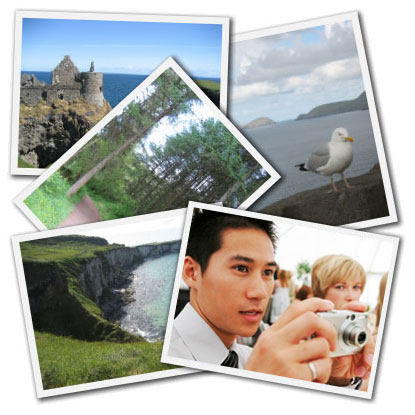
\includegraphics[height= 5cm]{images/collage.jpg}
\end{figure}
\end{frame}

\subsection{Key features}
\begin{frame}
\frametitle{Key features}
\begin{figure}
   
\includegraphics[height= 4cm]{images/resize.png}
\end{figure}
\end{frame}

\begin{frame}
\frametitle{Key features}
\begin{figure}
   
\includegraphics[height= 4cm]{images/rotate.png}
\end{figure}
\end{frame}

\begin{frame}
\frametitle{Key features}
\begin{figure}
   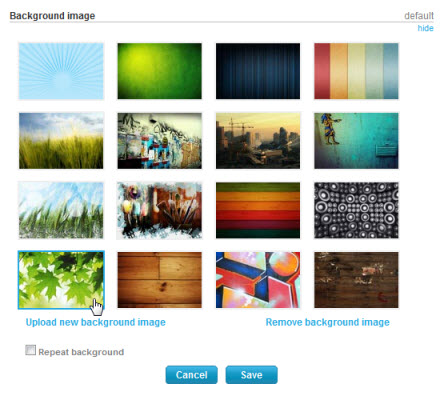
\includegraphics[height= 4cm]{images/change-background.jpg}
\end{figure}
\end{frame}

\begin{frame}
\frametitle{Key features}
\begin{figure}
   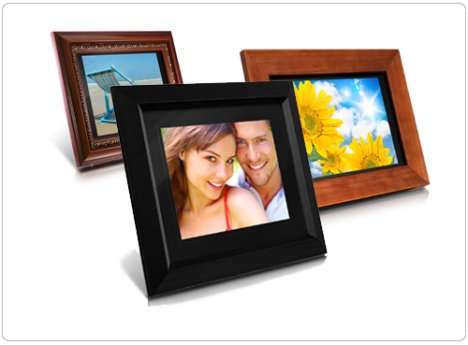
\includegraphics[height= 4cm]{images/photo-frame.jpg}
\end{figure}
\end{frame}

\begin{frame}
\frametitle{Key features}
\begin{figure}
   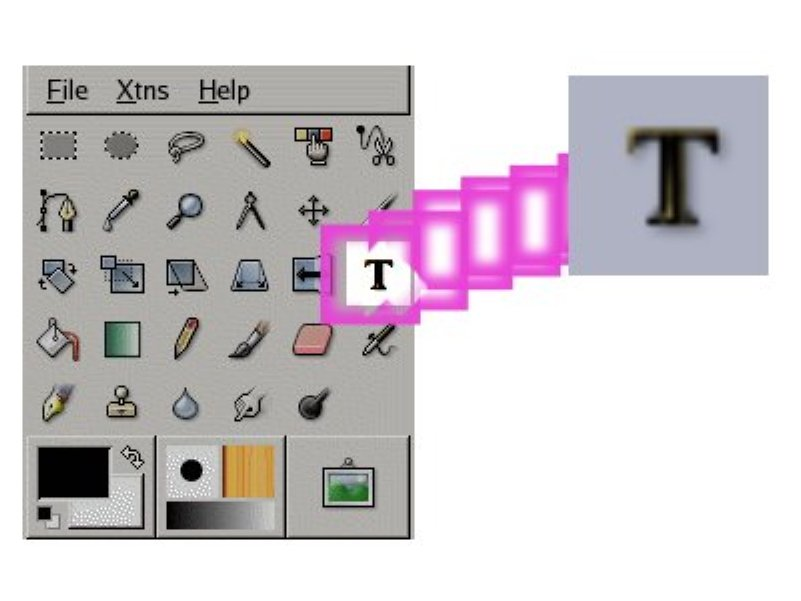
\includegraphics[height= 4cm]{images/text.jpg}
\end{figure}
\end{frame}

\section{Demo}
\begin{frame}
  \frametitle{Demo time}
  \framesubtitle{Hey! Look here! here!}
  \begin{alertblock}{!!!}
  \alert{Lets have a demo}\\ \pause
  Awesome, huh?
  \end{alertblock}
\end{frame}

\newcommand{\putlink}[1]{%
   \pgfsetlinewidth{1.4pt}%
   \pgfsetendarrow{\pgfarrowtriangle{4pt}}%
   \pgfline{\pgfxy(1,1)}{\pgfxy(#1,1)}
}

\begin{frame}
  \frametitle{Source code}
  \framesubtitle{If you want to improve the code}
  \begin{thebibliography}{10}

  \beamertemplatearticlebibitems

  \bibitem{beamer-homepage}
    Latest Source code of Collage Creator in Qt
    %\newblock {\tt \href{http://twitter.com/home}{Twitter}}
	\newblock{\url{https://bitbucket.org/seshagiriprabhu/qt_collage}}
	
  \bibitem{kdeslides}
    Latest source code of KIPI Collage Creator
%    \newblock {\tt }
	\newblock{\url{https://bitbucket.org/seshagiriprabhu/collage}}

  \end{thebibliography}
\end{frame}

\frame{
  \vspace{2cm}
  {\huge Questions ?}

  \vspace{3cm}
  \begin{flushright}
	Seshagiri Prabhu

    \structure{\footnotesize{seshagiriprabhu@gmail.com}}
  \end{flushright}
}

\end{document}
